\documentclass[tikz, border=10pt]{standalone}
\usepackage{tikz}
\usetikzlibrary{arrows.meta, positioning, shapes}

\tikzstyle{startstop} = [rectangle, rounded corners, draw, fill=black!0, text centered, minimum width=2cm, minimum height=1cm]
\tikzstyle{process} = [rectangle, draw, fill=black!20, text centered, minimum width=2cm, minimum height=0.75cm]
\tikzstyle{decision} = [diamond, draw, fill=black!10, text centered, aspect=1.5, inner sep=3pt]
\tikzstyle{arrow} = [thick, ->, >=stealth]

\newcommand{\windingTemperature}{{\vartheta}_{\mathrm{W}}}
\newcommand{\windingTemperatureMin}{{\vartheta}_{\mathrm{W,min}}}
\newcommand{\windingTemperatureMax}{{\vartheta}_{\mathrm{W,max}}}

\begin{document}

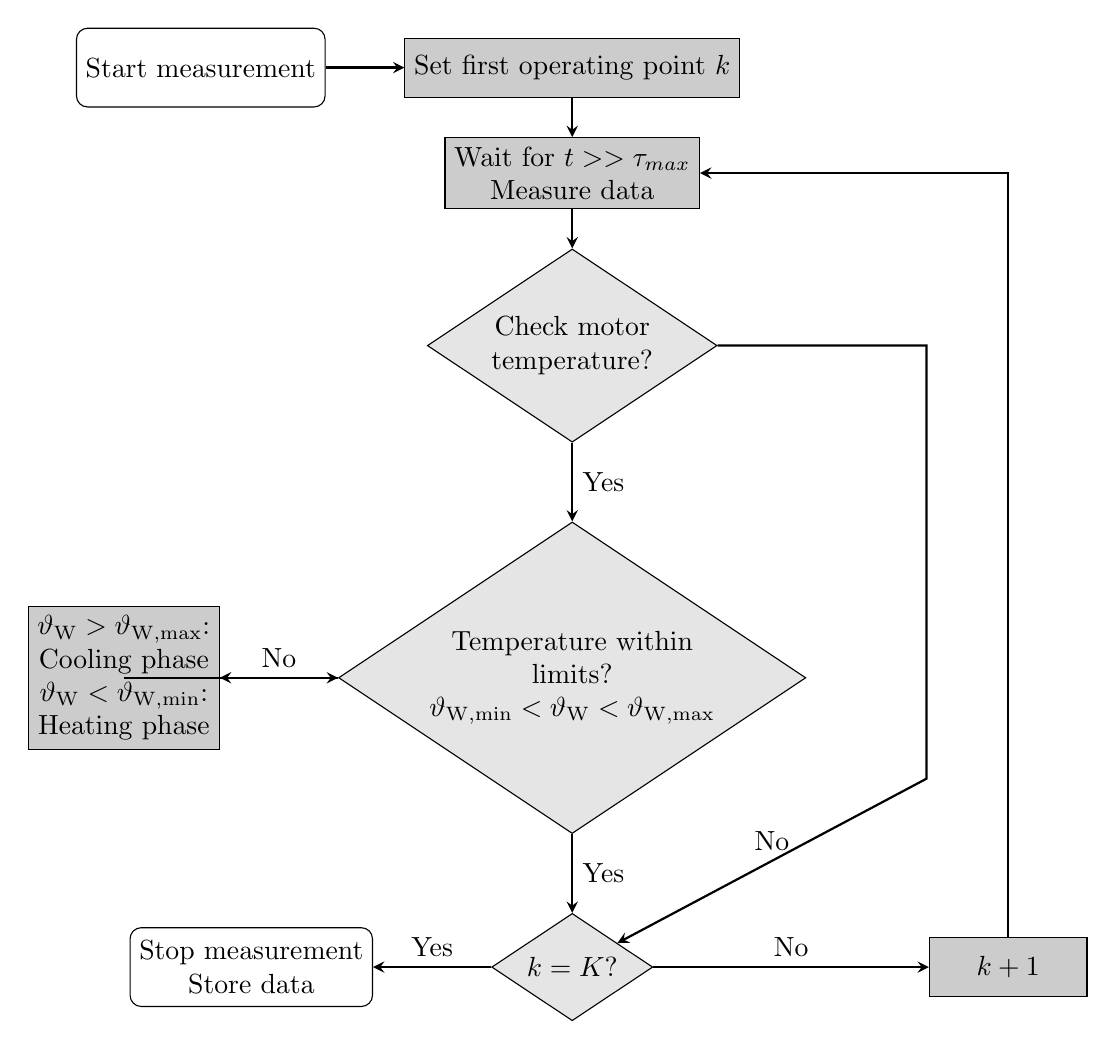
\begin{tikzpicture}[node distance=0.8cm]
% Nodes
\node (start) [startstop] {Start measurement};
\node (initialize) [process, right = 1cm of start, align=center]
{Set first operating point $k$};
\node (measure) [process, below = 0.5cm of initialize, align=center] {Wait for $t >> \tau_{max}$\\Measure data};

\node (tempavail) [decision, below = 0.5cm of measure, align=center] {Check motor \\ temperature?};

\node (tempcheck) [decision, below = 1cm of tempavail, align=center] {Temperature within \\ limits?\\ $\windingTemperatureMin < \windingTemperature < \windingTemperatureMax$};

\node (heating) [process, left=1.5cm of tempcheck, align=center] {$\windingTemperature > \windingTemperatureMax$:\\ Cooling phase\\ $\windingTemperature < \windingTemperatureMin$:\\ Heating phase};

\node (lastop) [decision, below=1cm of tempcheck, align=center]{$k=K$?};
\node (nextop) [process, right=3.5cm of lastop] {$k+1$};
\node (finish) [startstop, left=1.5cm of lastop, align=center] {Stop measurement\\Store data};

% Connections
\draw [arrow] (start) -- (initialize);
\draw [arrow] (initialize) -- (measure);
\draw [arrow] (measure) -- (tempavail);

\draw [arrow] (tempavail) -- node[right]{Yes} (tempcheck);
\draw [arrow] (tempavail) -- ++(4.5cm, 0cm) |- ++(0cm, -5.5cm) -- node[above]{No} (lastop);

\draw [arrow] (tempcheck) -- node[above]{No} (heating);
\draw [arrow] (heating) |- (tempcheck.west);

\draw [arrow] (tempcheck) -- node[right]{Yes} (lastop);

\draw [arrow] (lastop) -- node[above]{No} (nextop);
\draw [arrow] (nextop) |- (measure);
\draw [arrow] (lastop) -- node[above]{Yes} (finish);

\end{tikzpicture}

\end{document}
